% 
% This is a wrapper for component.tex.  It is used to build a standalone PDF
% file for just that component.
% 

\documentclass[11pt,letterpaper]{article}
% 1-inch margins all around
\usepackage[margin=1in]{geometry}
% Modern LaTeX font encoding
\usepackage[T1]{fontenc}
% Special characters from the main text font
\usepackage{textcomp}
% Change fonts to Times/Helvetica/Courier
\usepackage{mathptmx}
\usepackage[scaled=.92]{helvet}
\usepackage{courier}
\usepackage{color}
\usepackage[usenames,dvipsnames]{xcolor}
% \includegraphics
\usepackage{graphicx}
% \includepdf
\usepackage{pdfpages}
% \url (see below)
\usepackage{url}
% Compressed titles in sans-serif
\usepackage[sf,bf,compact]{titlesec}
% Captions that stand out from the text
\usepackage[small,bf]{caption}
% Sorted citations
\usepackage{cite}
% Compressed enumerations (see below)
\usepackage{enumitem}
% No indentation (see below)
\usepackage[parfill]{parskip}
% Include bibliography in index
\usepackage[nottoc,numbib]{tocbibind}
% \topcaption
%\usepackage{topcapt}
% \newcolumntype
\usepackage{dcolumn}
% Hyper references
%\usepackage[pdfborder={0 0 0}]{hyperref}
\usepackage{chapterfolder}

% Allow conditionals
\usepackage{ifthen}

\definecolor{lightgrey}{gray}{0.8}

% Set to false to hide comments
\newboolean{CommentsVisible}
\setboolean{CommentsVisible}{true}
\colorlet{commentbg}{SkyBlue}

% Show implementation details?
\newboolean{ImplementationDetailsVisible}
\setboolean{ImplementationDetailsVisible}{true}

% command to mark comments that are easily hidden
%\comment{this is a comment}
\ifthenelse{\boolean{CommentsVisible}}{%
\newcommand{\comment}[1]{%
\par%
\addvspace{\baselineskip}%
\noindent%
\fcolorbox{black}{commentbg}{%
\begin{minipage}{\textwidth}%
{\large \bf Review Comment}\\[2pt]%
#1%
\end{minipage}%
}%
\\[5pt]%
}}
%comments are not visible
{\newcommand{\comment}[1]{}}


%\newcommand{name of new command}[number of arguments]{definition} 
%\callout{indexname}{bgcolor}{leader}{shortname}{text}
\newcommand{\callout}[5]{%
\par%
\addvspace{\baselineskip}%
\noindent%
\index{#1}{#4}%
\fcolorbox{black}{#2}{%
\begin{minipage}{\textwidth}%
{\large \bf #3: #4 }\\[2pt]%
#5%
\end{minipage}%
}%
\\[5pt]%
}

%\todo{title}{text}
\makeindex{todo}
\newcommand{\todo}[2]{\callout{todo}{lightgrey}{TODO}{#1}{#2}}

%\assumption{title}{text}
\makeindex{assumptions}
\newcommand{\assumption}[2]{\callout{assumptions}{yellow}{Assumption}{#1}{#2}}

%\decision{title}{text}
\makeindex{decisions}
\newcommand{\decision}[2]{\callout{decisions}{yellow}{Decision Needed}{#1}{#2}}

%\detail{title}{text}
%\makeindex{detail}
\newcommand{\detail}[2]{%
\ifthenelse{\boolean{ImplementationDetailsVisible}}{%
\callout{detail}{lightgrey}{Implementation Detail}{#1}{#2}}{}}


% LaTeX is simply confused.  \frenchspacing should be the default, everywhere.
\frenchspacing

% URLs in sans-serif
\urlstyle{sf}



% Sane defaults for floats.
\renewcommand{\topfraction}{0.9}
\renewcommand{\bottomfraction}{0.9}
\renewcommand{\textfraction}{0.1}
\renewcommand{\floatpagefraction}{0.9}

\setcounter{topnumber}{2}
\setcounter{bottomnumber}{2}
\setcounter{totalnumber}{4}
\setcounter{dbltopnumber}{2}

% Bring figures closer to text
\renewcommand{\textfloatsep}{\intextsep}

% Remove needless spacing between the header and the first line.
\setlength{\topskip}{5pt}

% Reduce spacing between paragraphs in parskip
\setlength{\parskip}{5pt plus 1pt}

% Reduce spacing in itemize
\setitemize[1]{topsep=0pt,partopsep=0pt,itemsep=1pt,parsep=0pt,leftmargin=*}
%\setdescription{topsep=0pt,partopsep=0pt,itemsep=1pt,parsep=0pt}
\setdescription{topsep=0pt,partopsep=0pt,itemsep=1pt,parsep=0pt,leftmargin=10pt}

% Compute terms that LaTeX hyphenates badly by default
\hyphenation{off-loaded peta-scale exa-scale time-stamp}

% Generate PDF 1.6
\pdfoptionpdfminorversion=6

\pagestyle{empty}

\graphicspath{{./figures/}}

\begin{document}

\section{Streaming Translation Services}


\subsection{Proposed Architecture}

The purpose of the new Streaming Translation Service (STS) design is to enable
``near real-time delivery'' of experimental data to analysis, in the form of
both Event and Histogram NeXus files, within seconds or minutes of the
completion of a run.

\begin{figure}[htb]
\centering
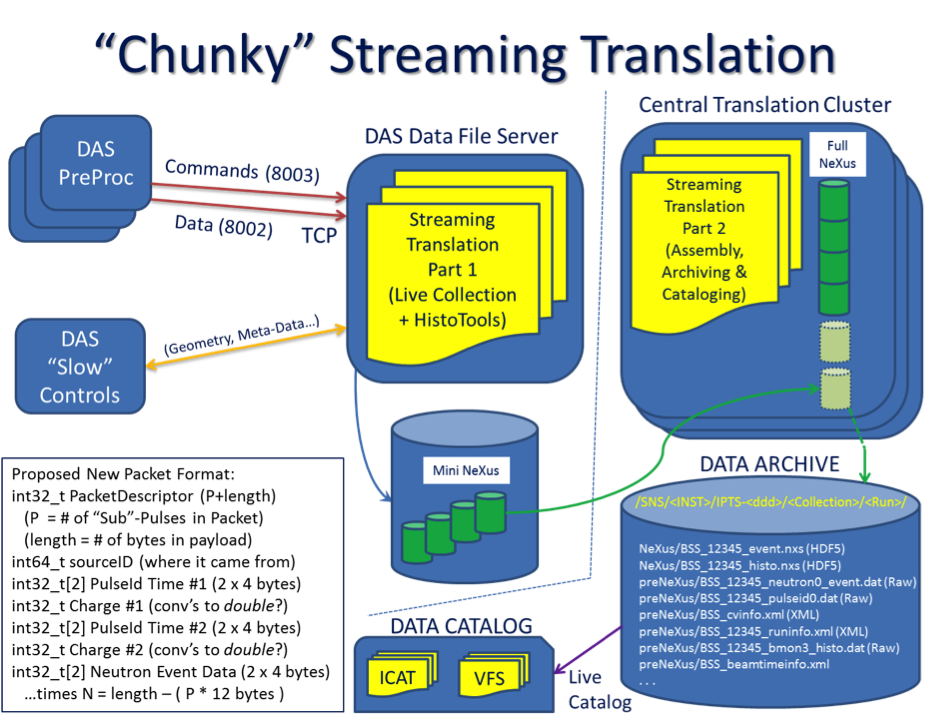
\includegraphics[width=5.5in]{chunky.png}
\caption{Initial ``Chunky'' Streaming Translation Architecture, Includes
generation of ``Mini-NeXus'' files for preliminary analysis and transport to
Central computing center.}
\label{fig:chunky_sts}
\end{figure}


\begin{figure}[htb]
\centering
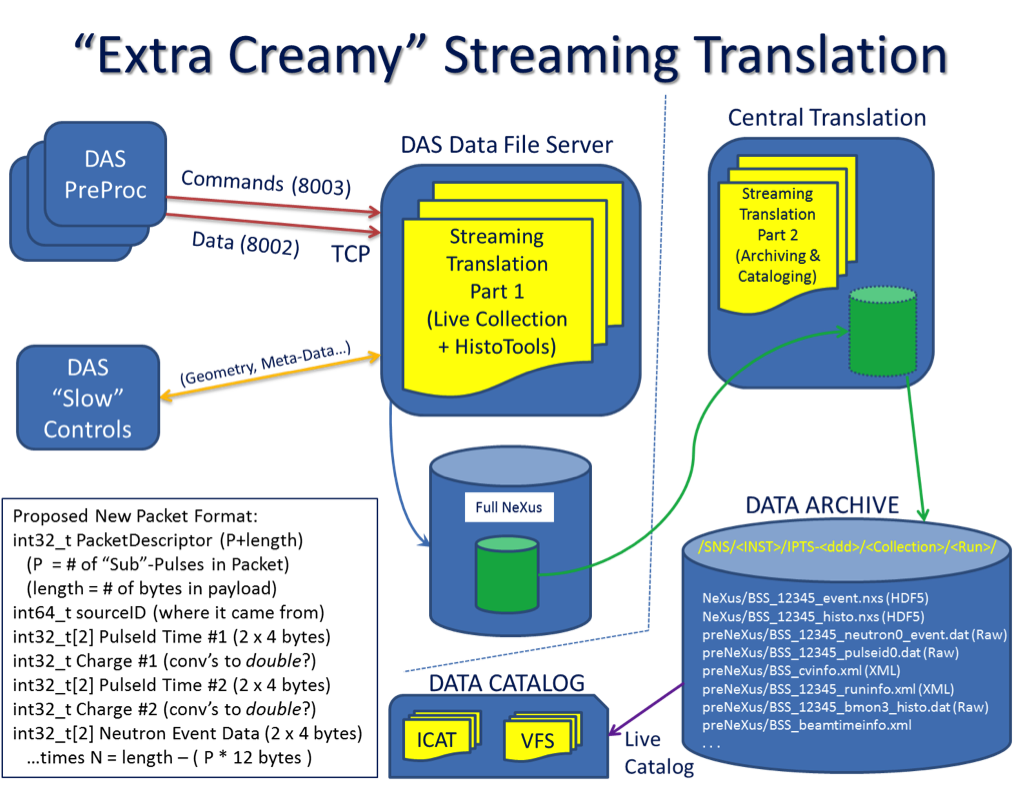
\includegraphics[width=5.5in]{creamy.png}
\caption{Effective Potential ``Extra Creamy'' Streaming Translation
Architecture, does Not include generation of ``Mini-NeXus'' files, only produces
a Full NeXus file for ``soon after post-mortem'' analysis, via transport (or
direct writing) to the Central computing center.}
\label{fig:creamy_sts}
\end{figure}


The basic proposed architecture for this STS design
is illustrated in Figures~\ref{fig:chunky_sts} and \ref{fig:creamy_sts},
for two incremental configurations based on use of intermediate
``Mini-NeXus'' file generation. Note that the actual boundary/separation between
the Data Acquisition System (DAS) and Central Computing Center is transient
here, and is expected to move as changes to the underlying network
infrastructure solidify. Yet moving or removing that boundary does not
fundamentally change the design elements or associated development tasks; e.g.
Parts 1 \& 2 of the Streaming Translation software can be combined into a
single Translation entity on the Central Computing side, without loss of
generality.


Much existing technology can be applied to assemble this new Streaming
Translation architecture, pulling code and expertise from each of the Live
Data Processing (LDP) ``Event Catcher'', the HistoTools Event- and
Histogram-based NeXus file generation applications \& library, and the
existing static Translation Service (TS) Client and TS Monitor GUI.  


In short, the intent is to attach an LDP ``front end'' onto a HistoTools
library ``back end'' to parse the Live Data Stream coming from the DAS and
generate Live Event (and Histogram) NeXus files while the experiment is
running. Based on existing technological capabilities, this Streaming
Translation solution should be able to adequately ``keep up'' with even the
highest bandwidth SNS beamline, and effectively be ``done'' creating a given
NeXus file (whether as a single monolithic file, or via the assembly of a
sequence of Mini-NeXus files) within moments after the last data packet
arrives, signaling the end of the experiment. Then the traditional Translation
Service Client can perform its usual Archiving and Cataloging services, along
with new extensions to improve performance, such as providing multi-threaded
concurrency in the translation processing to effectively ``overlap'' independent
operations and capitalize on powerful computational resources at SNS and
CCSD.

\subsubsection{Implementation Plan}

The STS implementation relies heavily on completion of the
Hybrid Streaming Network Protocol,
as described in Section~\ref{network_protocol}.
While some STS architectural re-organization and development can proceed
in unison with the design of the network protocol,
some practical results will be required early in the STS development.
Specifically, a ``Protocol Generator'' must be created to take existing
historical SNS data (likely in the ``Pre-NeXus'' binary format and the
associated XML meta-data files) and produce a network packet stream
using the new hybrid network protocol,
for proper design and testing of STS subsystems.
All specific packet types should be well defined,
including accelerator pulses, neutron events, beam monitor events,
chopper/special events, analog/pump probe sampling events,
polarization state transitions, slow controls meta-data/motor positions
(geometry) and accelerator information.
Beyond this preliminary stand-alone network protocol generator,
eventually a full ``side-by-side'' testbed should be provided,
in a real beamline hutch such as HYSPEC,
for testing in a production experimental environment.

The front-end of the new STS system will be derived from the
existing SNS production ``Live Data Processing'' (LDP)
Event Catcher software,
which is utilized to snoop packets from the legacy DAS live event stream
and incrementally produce transient ``Live'' histogram-based NeXus files
while an experiment is running.
An optional intermediate development step for STS would be to enable a
preliminary extension of the existing LDP stand-alone subsystem to produce
live {\em Event-based} ``Mini-NeXus'' files,
in preparation for subsequent potential STS needs.
These Mini-NeXus files {\em might} prove ``interesting'' or useful
for early Live Analysis developments.

Otherwise, the eventual plan for usage
of the current LDP Event Catcher infrastructure
would be as the front-end linkage between the new hybrid network protocol
and a back-end streaming HistoTools/Translation Service Client.
Based on the new network protocol,
a modified communication/control linkage will be incorporated
into the existing LDP network handler,
and then the new data stream can be captured and delivered appropriately
to the back-end client for processing
and collating the data into NeXus files.
This will require modified handling
for any beamline-specific geometry information,
which is currently extracted from a Live Geometry MySQL Database
in the existing Event Catcher software.
A migration must occur from this database infrastructure
to instead extract slow controls process variable updates
from the new network protocol packet types,
including all experiment-related meta-data on
users and proposal ids, in addition to motor positions, etc.

The back-end Streaming Translation Client (STC)
will itself consist of several subsystems,
also to be constructed from existing production SNS software projects,
namely the ``HistoTools'' NeXus file generation system
and the legacy static Translation Service Client.
The HistoTools application code and library can be applied,
by a straightforward manipulation of their current data input method,
to process a network stream instead of file based data.
This is especially feasible given the recent optimizations and
algorithmic reworking in the impending HistoTools 4.0.0 production release,
which processes input data using a ``pulse-driven'' mode
instead of an ``event-driven'' one.
This data handling approach,
while more efficient in terms of file-based processing,
is also directly amenable
to the processing of network packets in the new data protocol,
which are primarily pulse-driven with references to corresponding events.

A first step in this integration-based development
will be to effectively merge the LDP front end
with a proper HistoTools back end,
to replace the existing custom LDP NeXus file generation code
with linkage to the new HistoTools application/library.
An optional companion effort in this merging of LDP with HistoTools
would be to provide a common technology basis for
generating and merging ``partial'' Mini-NeXus files.
Any existing knowledge base for creating and managing Mini-NeXus files,
as generated in conjunction with the LDP Event Mini-NeXus option,
could be incorporated as part of the ``Chunky'' STS design.
A useful tool to create here, to aid development and testing,
is a ``file merger'' application/library,
for incrementally concatenating Mini-NeXus Files into
single monolithic NeXus files.
This tool development should include a full performance evaluation
and code ``hot-spot'' optimization exploration
to determine the feasibility of this approach in the STS overall design.
For example, an optimal ``chunk size'' for Mini-NeXus files
could be determined,
based on the overheads involved in concatenating them, etc.

The second key area of functionality in the STS back-end comes
from the existing production Translation Service (TS) Client software.
This software handles the notification of experiment completion,
and coordinates the execution of the HistoTools software applications
to produce Histogram and Event-based NeXus files.
The TS Client then archives and catalogs these files in ICAT and VFS,
along with the original raw experiment data and associated meta-data.
In the new STS design, many of these same tasks will still be required,
e.g. to properly archive and catalog the raw and processed experiment data.
But in the STS, data processing and NeXus file creation will proceed
{\em concurrently} with experimental data collection,
hence changing the nature of the completion notifications
and their handling.
The starting/stopping of data collection will now be handled
via direct communication in the hybrid network protocol,
using the ``Run Status'' packet type,
as part of the modified STS LDP/HistoTools linkage.
Similarly, the HistoTools back-end libraries will be continuously engaged
in data processing and creation of NeXus files,
rather than being triggered monotonically by the TS Client.
Yet the TS Client will still manage
the archiving and cataloging of experimental data,
including an additional new ``raw data'' file,
in the form of the captured network protocol stream,
which must also be written to local storage during processing.

Several additional features will be explored for improving the
capabilities, resilience and efficiency of the Translation Service Client
in this new STS back-end context.
New data products will be incorporated for ``Event Mode'' Beam Monitor data
and other ``Fast'' Meta-Data,
such as from Magnet Pulses on SEQUOIA
or High-Voltage/Analog Pump Probe on VULCAN.
Usage requirements for these emerging features
must be collected to ensure proper handling
and disposition of these specialized data products into NeXus files.

Because the existing production Translation Service Client
is used for a variety of experimental facilities beyond SNS,
including HFIR at ORNL,
it will be necessary to generalize/separate the workflow handling
of data for SNS versus HFIR and other facilities.
A new architecture for the Translation Service Client
will be designed, with specialized workflow handling for SNS,
while preserving the existing generic workflow for HFIR, LENS, etc.
The new STS Translation Service will also need to be enhanced
to interoperate with the impending ICAT3 database infrastructure,
for extended analysis meta-data searching and retrieval capabilities.

Finally, the Translation Service Client itself will be {\em optimized}
to allow more concurrency and flexibility in processing incoming data.
The current TS Client is primarily ``static'' in design,
and processes a {\em single} run at a time,
through all possible stages including final archiving and cataloging.
Yet indeed, often the processing of a given experiment run can get
bogged down in a specific stage, and hold up subsequent runs which
would otherwise be quickly and easily processed.
By dividing the TS Client processing into discrete ``pipeline stages''
and handling each stage independently
using its own pool of computational threads,
it will be easy for the TS Client to always ``make progress''
on trouble-free runs, even in the wake of other problematic runs
that have somehow gummed up the works.
Separate thread pools can be allocated for each type
of NeXus file post-processing,
e.g. to append Monitor histograms/events, beamline geometry,
or even for assembling ``complete'' NeXus files from Mini-NeXus elements.
Likewise, the sequential archiving and cataloging of the resulting
NeXus (and raw data) files can be decoupled into their own thread pools
and handled asynchronously.

Implicit in this new dynamic TS Client design
is the concept of ``processing state'',
which tracks the progress of each individual experimental run
through the post-processing pipeline.
A new database system will be enlisted to keep track
of each run's status and error conditions,
to provide a more meaningful overview of the full processing state.
This database will provide extended information
to the TS Monitor web application,
to more accurately show bottlenecks and processing problems,
and allow manual ``re-submission'' of failed pipeline stages.
Such a system would represent a fundamental improvement
over the existing ``all or nothing'' pass/fail TS Monitor reporting.

Integral to this detailed STS development
is proper capturing, handling and reporting of
System Status and Error conditions.
To emphasize the importance of this information
in the proper administration and maintenance
of the experimental facility,
consideration of Status/Error logging will be incorporated
early in the design of the new STS system.
An architecture will be designed for culminating status/error information
from across the DAS/Translation processing pipeline,
including both hardware and software errors,
as well as inherent data-related omissions or inconsistencies.
This status/error information must also be propagated
to a modified Translation Service Monitor
for easy notification and dissemination to support staff, end-users,
instrument scientists, and instrument hall coordinators.

Additional development may be explored to enable some rudimentary level of
automated recovery for handling streaming exceptions during an experiment,
e.g. regenerating key meta-data lost in the live stream,
using stream retry requests to the Data Aggregator
(which would pull a cached version of the stream from disk for replay).



\end{document}
